\chapter{Beschreibung des Endproduktes}\label{cha:theoretical-background}
\section{Administrion}
\subsection{Statistiken}
Um eine Übersicht über alle verkauften Brillen und Kontaktlinsen zu erhalten, gibt es einen Menüpunkt „Statistiken“. Dort wird ein Liniendiagramm der verkauften Brillen/Kontaktlinsen von diesem Jahr und dem Jahr davor angezeigt. Damit eine Brille/Kontaktlinse in der Statistik mitberücksichtigt wird, muss ein Zahlungsdatum angegeben werden und der Bezahlungsstatus muss auf „Bezahlt“ gesetzt werden.
\begin{figure}
\begin{center}
	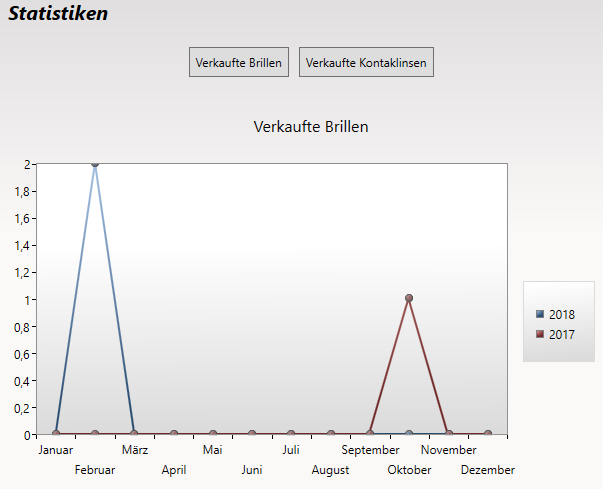
\includegraphics[scale=.4]{images/Statistiken.png}
\end{center}
	\caption{Screenshot der Statistiken}
	\label{fig:sample}
\end{figure}
\subsubsection{Technischer Hintergrund}
Zur Darstellung wurde das package System.Windows.Controls.DataVisualization.Toolkit 4.0.0 verwendet (wie oben beschrieben, Referenz einfügen). 
Dies wird folgendermaßen verwendet: 
In dem .xaml File muss der Namespace angegeben werden: 
\begin{lstlisting}
<Page xmlns:toolkitCharting="clr-namespace:System.Windows.Controls.DataVisualization.Charting;assembly=System.Windows.Controls.DataVisualization.Toolkit">
\end{lstlisting}
Um ein Liniendiagramm zu erzeugen:
\begin{lstlisting}
<toolkitCharting:Chart Title="{Binding Title}">
            <toolkitCharting:LineSeries Title="{Binding NewYear}"  DependentValueBinding="{Binding Value}" IndependentValueBinding="{Binding Key}" ItemsSource="{Binding NewValues}"/>
            <toolkitCharting:LineSeries Title="{Binding OldYear}"  DependentValueBinding="{Binding Value}" IndependentValueBinding="{Binding Key}" ItemsSource="{Binding OldValues}"/>
        </toolkitCharting:Chart>
\end{lstlisting}
Dabei sind "NewValues" und "OldValues" vom Typ: 
\begin{lstlisting}
        public ObservableCollection<KeyValuePair<string, int>> NewValues { get; set; }
        public ObservableCollection<KeyValuePair<string, int>> OldValues { get; set; }
\end{lstlisting}
Die Daten werden mittels Linq(Referenz) erfasst.